\documentclass[tikz,border=5pt]{standalone}
\usepackage{amsmath}
\usetikzlibrary{arrows.meta,calc,decorations.pathreplacing}
\definecolor{ink}{HTML}{16324F}
\definecolor{teal}{HTML}{168A88}
\definecolor{gold}{HTML}{D9892B}
\definecolor{soft}{HTML}{EAF5F4}
\begin{document}
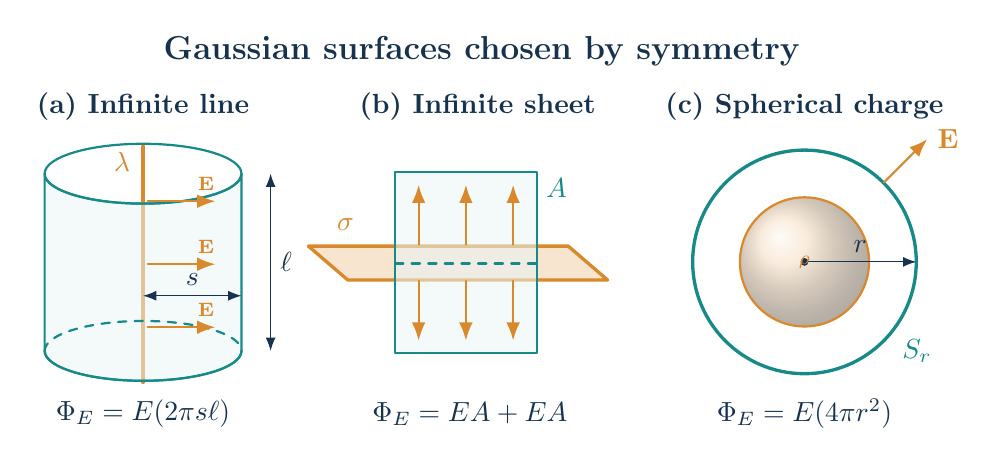
\begin{tikzpicture}[font=\sffamily,>=Latex,line cap=round,line join=round]
  \node[font=\bfseries\large,ink] at (6.1,4.55) {Gaussian surfaces chosen by symmetry};

  % Infinite line
  \begin{scope}[shift={(0,0)}]
    \node[font=\bfseries,ink] at (1.8,3.85) {(a) Infinite line};
    \draw[gold,very thick] (1.8,0.35)--(1.8,3.35);
    \node[gold,left] at (1.76,3.15) {$\lambda$};
    \draw[teal,thick,fill=soft,fill opacity=.55] (.55,.75) arc[start angle=180,end angle=360,x radius=1.25,y radius=.38]
      -- (3.05,3.00) arc[start angle=0,end angle=-180,x radius=1.25,y radius=.38] -- cycle;
    \draw[teal,thick] (.55,3.00) arc[start angle=180,end angle=540,x radius=1.25,y radius=.38];
    \draw[teal,thick,dashed] (.55,.75) arc[start angle=180,end angle=0,x radius=1.25,y radius=.38];
    \draw[teal,thick] (.55,.75) arc[start angle=180,end angle=360,x radius=1.25,y radius=.38];
    \draw[<->,ink] (1.8,1.45)--(3.05,1.45) node[midway,above] {$s$};
    \draw[<->,ink] (3.42,.75)--(3.42,3.00) node[midway,right] {$\ell$};
    \foreach \y in {1.05,1.85,2.65}{
      \draw[->,gold,thick] (1.86,\y)--(2.72,\y) node[pos=.86,above] {\scriptsize$\mathbf E$};
    }
    \node[align=center,ink] at (1.8,-.05) {$\Phi_E=E(2\pi s\ell)$};
  \end{scope}

  % Infinite sheet
  \begin{scope}[shift={(4.15,0)}]
    \node[font=\bfseries,ink] at (1.9,3.85) {(b) Infinite sheet};
    \fill[gold!22] (.25,1.65)--(3.55,1.65)--(3.05,2.08)--(-.25,2.08)--cycle;
    \draw[gold,very thick] (.25,1.65)--(3.55,1.65)--(3.05,2.08)--(-.25,2.08)--cycle;
    \node[gold] at (.22,2.35) {$\sigma$};
    \draw[teal,thick,fill=soft,fill opacity=.55] (.85,.72) rectangle (2.65,3.02);
    \draw[teal,thick,dashed] (.85,1.86)--(2.65,1.86);
    \node[teal] at (2.9,2.82) {$A$};
    \foreach \x in {1.15,1.75,2.35}{
      \draw[->,gold,thick] (\x,2.10)--(\x,2.86);
      \draw[->,gold,thick] (\x,1.64)--(\x,.88);
    }
    \node[align=center,ink] at (1.8,-.05) {$\Phi_E=EA+EA$};
  \end{scope}

  % Sphere
  \begin{scope}[shift={(8.45,0)}]
    \node[font=\bfseries,ink] at (1.75,3.85) {(c) Spherical charge};
    \shade[ball color=gold!45,opacity=.48] (1.75,1.88) circle (.82);
    \draw[gold,thick] (1.75,1.88) circle (.82);
    \draw[teal,very thick] (1.75,1.88) circle (1.42);
    \fill[ink] (1.75,1.88) circle (1.4pt);
    \draw[->,ink] (1.75,1.88)--(3.17,1.88) node[midway,above] {$r$};
    \draw[->,gold,thick] (2.76,2.89)--(3.31,3.44) node[right] {$\mathbf E$};
    \node[gold] at (1.75,1.88) {\scriptsize\(\rho\)};
    \node[teal] at (3.18,.75) {$S_r$};
    \node[align=center,ink] at (1.75,-.05) {$\Phi_E=E(4\pi r^2)$};
  \end{scope}
\end{tikzpicture}
\end{document}
